\documentclass[12pt]{article}
\usepackage{amsmath}
\usepackage[margin=1in]{geometry}
\usepackage{tikz} % For TikZ diagrams
\usetikzlibrary{shapes,arrows} % TikZ libraries

% TikZ styles
\tikzstyle{input} = [coordinate]
\tikzstyle{output} = [coordinate]
\tikzstyle{sum} = [draw, circle, node distance=1.5cm, inner sep=6pt]
\tikzstyle{block} = [draw, rectangle, minimum height=2em, minimum width=2.5em]

\begin{document}

\section*{Problem \#1}
The following Forward path Transfer Functions are given:

\begin{flalign}
  (a) \quad G(s) &= \frac{K}{(1+s)(1+10s)(1+20s)} && \notag \\
  (b) \quad G(s) &= \frac{10e^{-0.2s}}{(1+s)(1+10s)(1+20s)} && \notag \\
  (c) \quad G(s) &= \frac{10(s+1)}{s(s+5)(s+6)} && \notag \\
  (d) \quad G(s) &= \frac{100(s-1)}{s^2(s+5)(s+6)^2} && \notag \\
  (e) \quad G(s) &= \frac{10(s+1)}{s^3(s^2 + 5s + 5)} && \notag \\
  (f) \quad G(s) &= \frac{100}{s^3(s+2)^2} && \notag \\
  (g) \quad G(s) &= \frac{5(s+2)}{s^2(s+4)} && \notag \\
  (h) \quad G(s) &= \frac{8(s+1)}{(s^2 + 2s + 3)(s+1)} && \notag
\end{flalign}
\subsection*{Objective}
For the unity-feedback control systems described above, determine the steady-state error for:
\begin{itemize}
  \item A unit-step input
  \item A unit-ramp input
  \item A parabolic input, \( \dfrac{t^2}{2} u_s(t) \)
\end{itemize}
Check the stability of the system before applying the final-value theorem.

\newpage

\section*{Problem \#2}
The following single-loop nonunity-feedback control system transfer functions are given: 

\begin{flalign}
(a) \quad G(s) &= \frac{1}{s^2 + s + 2} & H(s) &= \frac{1}{s + 1} && \notag \\
(b) \quad G(s) &= \frac{1}{s(s + 5)} & H(s) &= 5 && \notag \\
(c) \quad G(s) &= \frac{1}{s^2(s + 10)} & H(s) &= \frac{s + 1}{s + 5} && \notag \\
(d) \quad G(s) &= \frac{1}{s^2(s + 12)} & H(s) &= 5(s + 2) && \notag
\end{flalign}

\subsection*{Objective}
For the systems above, calculate the steady-state errors for the following types of inputs:
\begin{itemize}
    \item Unit-step input
    \item Unit-ramp input
    \item Parabolic input given by \( \dfrac{t^2}{2} u_s(t) \)
\end{itemize}

\newpage
\section*{Problem \#3}

\subsection*{Description}
The Block Diagram of a control system is shown below.

\subsection*{Block Diagram}

\begin{center}
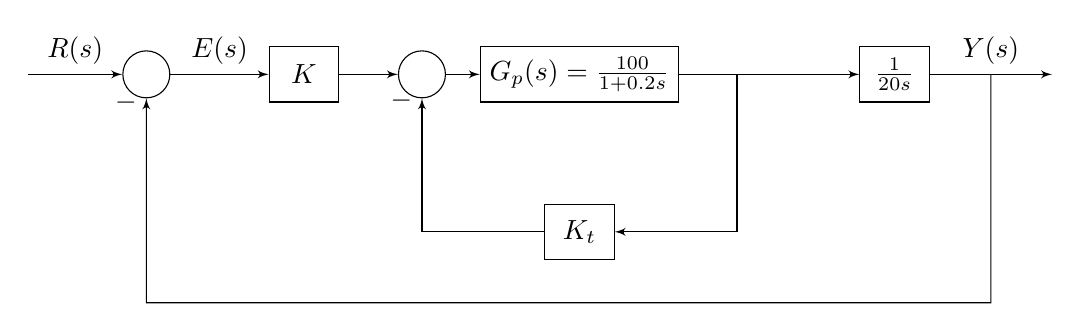
\begin{tikzpicture}[scale=0.8, auto, node distance=2cm,>=latex']
    % Drawing blocks and nodes
    \node [input, name=input] {};
    \node [sum, right of=input] (sum1) {};
    \node [block, right of=sum1] (K) {$K$};
    \node [sum, right of=K] (sum2) {};
    \node [block, right of=sum2] (Gp) {$G_p(s) = \frac{100}{1 + 0.2s}$};
    \coordinate[right of=Gp] (middle);
    \node [block, right of=middle] (sys) {$\frac{1}{20s}$};
    \node [output, right of=sys] (output) {};
    \node [block, below of=Gp] (Kt) {$K_t$};
    
    % Connectors
    \draw [draw,->] (input) -- node {$R(s)$} (sum1);
    \draw [->] (sum1) -- node {$E(s)$} (K);
    \draw [->] (K) -- node {} (sum2);
    \draw [->] (sum2) -- node {} (Gp);
    \draw [-] (Gp) -- node {} (middle);
    \draw [->] (middle) -- node {} (sys);
    \draw [->] (sys) -- node [name=Y] {$Y(s)$} (output);
    \draw [->] (middle) |- (Kt);
    \draw [->] (Kt) -| node[pos=0.99, left] {$-$} (sum2);
    \draw [->] (Y) -- ++ (0,-4) -| node[pos=0.99] {$-$} 
        node [near end] {} (sum1);
\end{tikzpicture}
\end{center}

\subsection*{Objective}
\subsubsection*{Task 1: Error Constants}
Determine the following error constants for the control system:
\begin{itemize}
    \item Step-error constant
    \item Ramp-error constant
    \item Parabolic-error constant
\end{itemize}
The error signal in the system is defined as \(e(t)\).

\subsubsection*{Task 2: Steady-State Errors}
Calculate the steady-state errors for the control system, assuming it is stable. The steady-state errors should be expressed in terms of \(K\) and \(K_t\). Perform these calculations for the following input functions:

\begin{enumerate}
    \item \( r(t) = u_s(t) \)
    \item \( r(t) = tu_s(t) \)
    \item \( r(t) = \frac{t^2}{2}u_s(t) \)
\end{enumerate}
\newpage
\section*{Problem 4}

The unit-step response of a linear control system is shown in the Figure.

\begin{figure}[h]
    \centering
    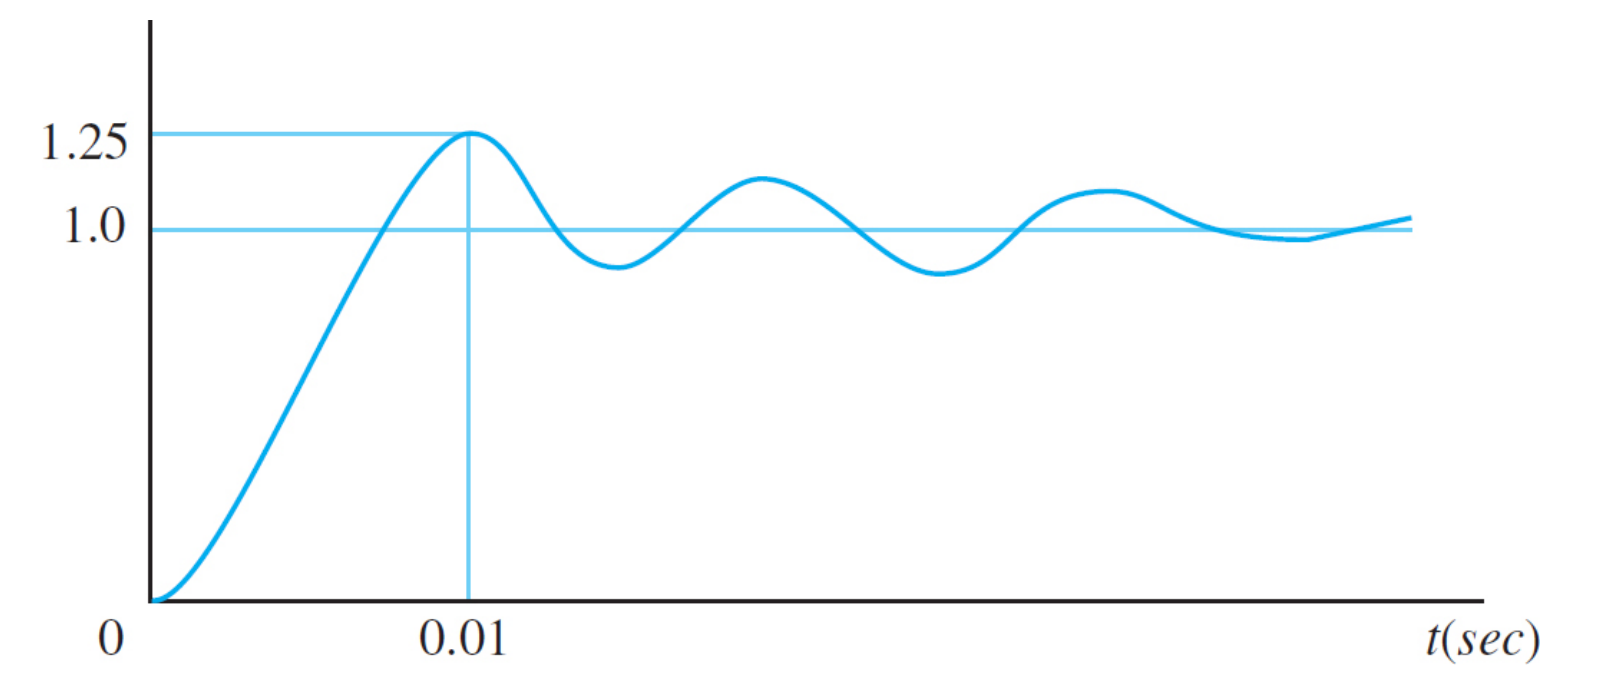
\includegraphics[width=0.8\linewidth]{Figure_P4.png} % replace 'path_to_your_figure.png' with your actual path and filename
    \caption{Unit-step response of the control system.}
    \label{fig:unit_step_response}
\end{figure}
\subsection*{Objective}
\noindent Find the transfer function of a second-order prototype system to model the system.
\newpage

\section*{Problem \#5}

A control system is shown below:
\subsection*{Block Diagram}

\begin{center}
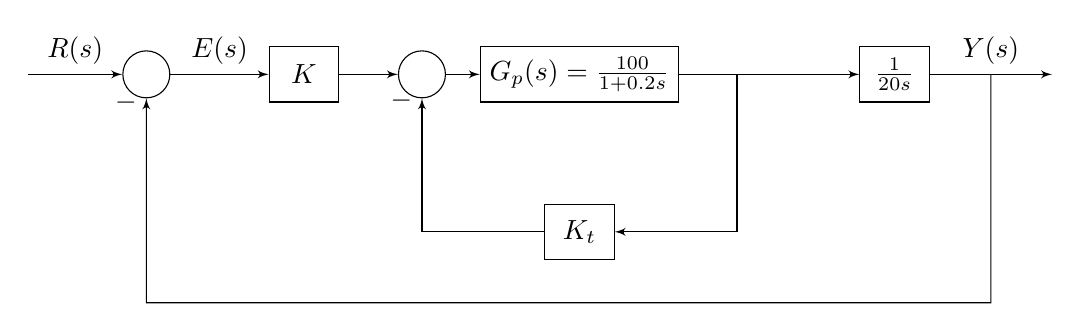
\begin{tikzpicture}[scale=0.8, auto, node distance=2cm,>=latex']
    % Drawing blocks and nodes
    \node [input, name=input] {};
    \node [sum, right of=input] (sum1) {};
    \node [block, right of=sum1] (K) {$K$};
    \node [sum, right of=K] (sum2) {};
    \node [block, right of=sum2] (Gp) {$G_p(s) = \frac{100}{1 + 0.2s}$};
    \coordinate[right of=Gp] (middle);
    \node [block, right of=middle] (sys) {$\frac{1}{20s}$};
    \node [output, right of=sys] (output) {};
    \node [block, below of=Gp] (Kt) {$K_t$};
    
    % Connectors
    \draw [draw,->] (input) -- node {$R(s)$} (sum1);
    \draw [->] (sum1) -- node {$E(s)$} (K);
    \draw [->] (K) -- node {} (sum2);
    \draw [->] (sum2) -- node {} (Gp);
    \draw [-] (Gp) -- node {} (middle);
    \draw [->] (middle) -- node {} (sys);
    \draw [->] (sys) -- node [name=Y] {$Y(s)$} (output);
    \draw [->] (middle) |- (Kt);
    \draw [->] (Kt) -| node[pos=0.99, left] {$-$} (sum2);
    \draw [->] (Y) -- ++ (0,-4) -| node[pos=0.99] {$-$} 
        node [near end] {} (sum1);
\end{tikzpicture}
\end{center}
\subsection*{Objective}
Find the values of \( K \) and \( K_t \) so that the maximum overshoot of the output is approximately \( 10\% \) and the rise time \( t_r \) is approximately \( 0.1 \, \text{s} \). Use 
\[
\omega_n \sqrt{1 - \xi^2} t = n\pi, \quad \text{where } n = 0, 1, 2, 3, \ldots
\]
for the rise-time relationship.
\newline \newline
\noindent Simulate the system with MATLAB to check the accuracy of your solutions.

\newpage
\section*{Problem \#6}

A control system is shown below:
\subsection*{Block Diagram}

\begin{center}
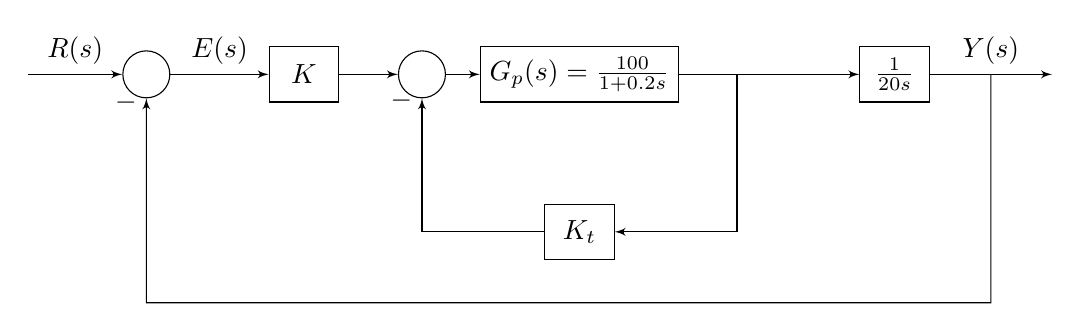
\begin{tikzpicture}[scale=0.8, auto, node distance=2cm,>=latex']
    % Drawing blocks and nodes
    \node [input, name=input] {};
    \node [sum, right of=input] (sum1) {};
    \node [block, right of=sum1] (K) {$K$};
    \node [sum, right of=K] (sum2) {};
    \node [block, right of=sum2] (Gp) {$G_p(s) = \frac{100}{1 + 0.2s}$};
    \coordinate[right of=Gp] (middle);
    \node [block, right of=middle] (sys) {$\frac{1}{20s}$};
    \node [output, right of=sys] (output) {};
    \node [block, below of=Gp] (Kt) {$K_t$};
    
    % Connectors
    \draw [draw,->] (input) -- node {$R(s)$} (sum1);
    \draw [->] (sum1) -- node {$E(s)$} (K);
    \draw [->] (K) -- node {} (sum2);
    \draw [->] (sum2) -- node {} (Gp);
    \draw [-] (Gp) -- node {} (middle);
    \draw [->] (middle) -- node {} (sys);
    \draw [->] (sys) -- node [name=Y] {$Y(s)$} (output);
    \draw [->] (middle) |- (Kt);
    \draw [->] (Kt) -| node[pos=0.99, left] {$-$} (sum2);
    \draw [->] (Y) -- ++ (0,-4) -| node[pos=0.99] {$-$} 
        node [near end] {} (sum1);
\end{tikzpicture}
\end{center}

\subsection*{Objective}
Find the values of \( K \) and \( K_t \) so that the maximum overshoot of the output is approximately \( 4.3\% \) and the delay time \( t_d \) is approximately \( 0.1 \, \text{s} \). Use 
\[
\frac{dy(t)}{dt} = \frac{\omega_n e^{-\xi \omega_n t}}{\sqrt{1 - \xi^2}} \left[ \xi \sin(\omega t + \theta) - \sqrt{1 - \xi^2} \cos(\omega t + \theta) \right], \quad \text{when } t \geq 0
\]
for the delay-time relationship.
\newline \newline
\noindent Simulate the system with MATLAB to check the accuracy of your solutions.
\newpage
\section*{Problem \#7}
The Figure shows the block diagram of a servomotor.
\subsection*{Block Diagram}
\begin{center}
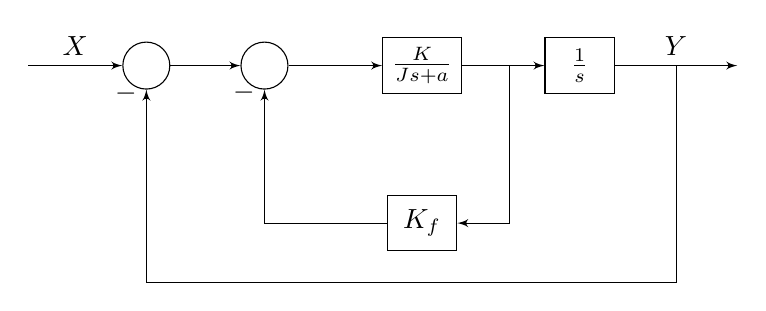
\begin{tikzpicture}[scale=1.2, auto, node distance=2cm,>=latex']
    % Define the nodes
    \node [input, name=input] {};
    \node [sum, right of= input] (sum1) {};
    \node [sum, right of= sum1] (sum2) {};
    \node [block, right of= sum2] (block1) {$\frac{K}{Js+a}$};
    \node [block, right of= block1] (block2) {$\frac{1}{s}$};
    \node [output, right of= block2] (output) {};
    \node [block, below of= block1] (block3) {$K_f$};
    % Connect the nodes
    \draw [->] (input) -- node[name=X] {$X$} (sum1);
    \draw [->] (sum1) -- (sum2);
    \draw [->] (sum2) -- (block1);
    \draw [->] (block1) -- (block2);
    \draw [->] (block2) -- node[name=Y] {$Y$} (output);
    \draw [->] (block1.east) -- ++(0.5cm,0) |- (block3);
    \draw [->] (block3) -| node[pos=0.99] {$-$} node [near end, left] {} (sum2);
    \draw [->] (Y) |- ++(0,-2.5cm) -| node[pos=0.99] {$-$} node [near end, right] {} (sum1);
\end{tikzpicture}
\end{center}
\subsection*{Objective}

\noindent Assume \( J = 1 \) kg-m\(^2\) and \( B = 1 \) N \( \cdot \) m/rad/s. If the maximum overshoot of the unit-step input and the peak time are 0.2 and 0.1 s, respectively,

\begin{enumerate}
    \item Find its damping ratio and natural frequency.
    \item Find the gain \( K \) and velocity feedback \( K_f \). Also, calculate the rise time and settling time.
\end{enumerate}




\end{document}
